\documentclass[a4paper]{article} % база.

%Пакеты для математических символов:
\usepackage{amsmath} % американское математическое сообщество.
\usepackage{amssymb} % миллион разных значков и готический, ажурный шрифты.
\usepackage{amscd} % диаграммы, графики.
\usepackage{amsthm} % окружения теорем, определений и тд.
\usepackage{latexsym} % треугольники и пьяная стрелка.

%пакеты для шрифтов:
\usepackage{euscript} % прописной шрифт с завитушками.
\usepackage{textcomp} % странные, но смешные значки(есть значок листика).
\usepackage{verbatim} % улучшенный шрифт "пишущей машинки".
\usepackage{array} % более удобные таблицы.
\usepackage{multirow} % мультистолбцы в таблицах.
\usepackage{longtable} % таблицы на несколько страниц.

%Пакеты для оформления:
\usepackage[x11names]{xcolor} % 317 новых цветов для текста.
\usepackage[unicode, pdftex]{hyperref} % гиперссылки
\usepackage{multicol} % набор текста в несколько колонн.
\usepackage{graphicx} % расширенные возможности вставки стандартных картинок.
\usepackage{subcaption} % возможность вставлять картинки в строчку
\usepackage{wrapfig} % вставка картинок и таблиц, обтекаемых текстом.
\usepackage{cancel} % значки для сокращения дробей, упрощения, стремления.
\usepackage{misccorr} % в заголовках появляется точка, но при ссылке на них ее нет.
%\usepackage{indentfirst} % отступ у первой строки раздела
%\usepackage{showkeys} % показывает label формул над их номером.
\usepackage{fancyhdr} % удобное создание верхних и нижних колонтитулов.
%\usepackage{titlesec} % еще одно создание верхних и нижних колонтитулов
\usepackage{titlesec}
\usepackage[font=Large,floatrowsep=qquad, captionskip=5pt]{floatrow}

%Пакеты шрифтов, кодировок. НЕ МЕНЯТЬ РАСПОЛОЖНИЕ.
\usepackage[utf8]{inputenc} % кодировка символов.
\usepackage{mathtext} % позволяет использовать русские буквы в формулах. НеОВМеТИМО С tempora.
\usepackage[T1, T2A]{fontenc} % кодировка шрифта.
\usepackage[english, russian]{babel} % доступные языки.
%\usepackage{tempora} % новый шрифт tempora.
%\usepackage{newtxmath} % новый шрифт tempora для формул.
\usepackage{anyfontsize} % масштабирует шрифты до необходимых размеров.

%Отступы и поля:
%размеры страницы А4 11.7x8.3in
\textwidth=7.3in % ширина текста
\textheight=10in % высота текста
\oddsidemargin=-0.5in % левый отступ(базовый 1дюйм + значение)
\topmargin=-0.5in % отступ сверху до колонтитула(базовый 1дюйм + значение)

\titleformat{\section}
{\normalfont\fontsize{21}{12}\bfseries \vspace{2.5mm}}{\thesection}{0.6em}{}
\titleformat{\subsection}
{\normalfont\fontsize{18}{12}\bfseries}{\thesubsection}{0.6em}{}
\renewcommand{\baselinestretch}{1.4}
\floatsetup[figure]{style=plaintop}
\usepackage{indentfirst}

%Настройки шапки у страниц
\pagestyle{fancy}
\fancyhead{}
\fancyhead[LE, RO]{\fontsize{14pt}{11pt}\selectfont \thepage}
\fancyhead[CO]{}
\fancyhead[LO]{\fontsize{14pt}{11pt}\selectfont Точки Лагранжа} 
\fancyhead[CE]{\fontsize{14pt}{11pt}\selectfont Точки Лагранжа} 
\fancyfoot{}

%Всякая дичь:
\relpenalty=10000 % бан на перенос на следующую строку внутри текста.
\binoppenalty=10000 % бан на перенос на следующую строку внутри.
\clubpenalty=10000 % бан на перенос первой строки абзаца на следующую страницу.
\widowpenalty=10000 % бан на перенос последней строки абзаца на следующую страницу.
%\emergencystretch=25pt % более качественные переносы слов. 
\setcounter{MaxMatrixCols}{25} % максимальный размер матрицы 25х25.

%Новые команды:
\newcommand*{\parfrac}[3]{\ensuremath{\left( \frac{ \partial #1}{\partial #2} \right)_{#3}}} % частная производная. #1 - числитель, #2 - знаменатель, #3 - постоянный параметр.
\newcommand*{\tx}[1]{\text{#1}} % сокращение для \text.
\newcommand*{\nnd}{\noindent} % сокращение для \noindent

%Определение математических операторов:
\DeclareMathOperator{\arch}{arch} %гиперболический ареакосинус.
\DeclareMathOperator{\arsh}{arsh} %гиперболический ареасинус.
\DeclareMathOperator{\arth}{arth} %гиперболический ареатангенс.
\DeclareMathOperator{\arcth}{arcth} %Гиперболический ареакотангенс.

%Переопределение команд:
\renewcommand{\labelenumi}{\theenumi)} % счетчик нумеруется в виде 1).
\renewcommand{\theenumii}{\arabic{enumii}} % счетчик нумеруется цифрами.
\renewcommand{\labelenumii}{\theenumii)} % уровень вложенности 2.
\newcommand{\theenumiii}{\arabic{enumiii}} % уровень вложенности 3.
\renewcommand{\labelenumiii}{\theenumiii)}

\begin{document}

	\fontsize{14pt}{11.75pt}\selectfont
	
	\begin{titlepage}
		\begin{center}

			\includegraphics[width=90mm]{title.png}
			\vspace{5mm}
			
			{\Huge Московский физико-технический институт}
			
			\vspace{5mm}
			{\LARGE Вопрос по выбору}
			
			\vspace{6mm}
			\noindent\rule{15cm}{0.5pt}
			
			\vspace{2mm}
			{\Huge \textbf{Точки Лагранжа. \linebreak Положение, устойчивость равновесия и применение}}
			\vspace{-2mm}
			
			\noindent\rule{15cm}{0.5pt}
			
			{\Large \begin{multicols}{2}
					\textit{}
					
					\textit{Семестр:} 1 \\ \
					
					\textit{Работу выполнил:} \\ Степанов Тимофей
					
					\textit{Группа:} Б02-308
					
			\end{multicols}}
		\end{center}
		%\begin{abstract}
		%Данная работа направлена на теоретический расчет положения точек Лагранжа и анализ устойчивости положения в них
		%\end{abstract}
	\end{titlepage}
	
\section{Определение}

\textbf{Ограниченной задачей трех тел} называют частный случай задачи трех тел, когда масса одного из тел достаточно мала, чтобы его влиянием на два других можно было пренебречь. В этом случае два тела большей массы будут двигаться тому как они двигаться в задаче двух тел, а 3-е двигаться под влиянием двух других.

\textbf{Точками Лагранжа} называют точки в системе ограниченной задачи трех тел движущихся по круговой траектории, в которых меньшее тело будет оставаться неподвижным относительно 2-х других.

Прежде чем рассматривать систему трех тел следует получить несколько фактов о характере движения двух тел.

\section{Задача двух тел}

%\textbf{Утвержение 1:} Два гравитирующих тела будут вращаться вокруг центра масс и их угловая скорость одинакова.

%Т.к. мы рассматриваем изолированную систему, ускорение центра масс будет равно 0, т.е. система отсчета связанная с центром масс - инерциальная. Теперь пусть в системе центра масса одно из тел сдвинулась на малый угол. Тогда второе тело будет лежать на прямой, соединяющей первое тело и центр масс, который в собственной системе неподвижен. Тогда из вертикальности углов следует, что второе тело сдвинулась на тот же угол, откуда следует равенство угловых скоростей.\\

%\nnd \textbf{Утверждение 2:} Для системы двух гравитирующих тел выполняется $\Omega^2 R^3 = G(m_1 + m_2)$, где $\Omega$ - угловая скорость тел планет вокруг центра масс, $R$ - расстояние между телами, $m_1, m_2$ - массы тел

Покажем, что два изолированных гравитирующих тела будут вращаться вокруг своего центра масс с одинаковой угловой сокростью $\Omega$.

Введем неподвижную систему отсчета с началом в точке $O$. Пусть $\vec{r_{1,2}}$ - радиус-векторы тел, $\vec{r_g}$ - радиус вектор центра масс.

Введем $\vec{r} = \vec{r_2} - \vec{r_1}$. Тогда второй закон Ньютона для каждого из тел запишется как:
\begin{equation}
m_1\ddot{\vec{r_1}} = G\frac{m_1 m_2}{r^2}\vec{e_r};\text{ }m_2\ddot{\vec{r_2}} = -G\frac{m_1 m_2}{r^2}\vec{e_r} 
\end{equation}
Тогда
\begin{equation}
\ddot{\vec{r}} = \ddot{\vec{r_2}} - \ddot{\vec{r_1}} = -G\frac{m_1 + m_2}{r^2}\vec{e_r}
\end{equation}
Это можно выражение можно записать как:
\begin{equation}
m_1\ddot{\vec{r}} = -\frac{\mu}{r^2}m_1\vec{e_r}
\label{3}
\end{equation}
где $\mu = G(m_1 + m_2)$.

Для понимания физического смысла полученного выражения следует ввести понятие Кеплеровой задачи. \textbf{Кеплерова задача} - задача о движении тела в инерциальной системе отсчета, начало которой совпадает с "источником" центрального поля силы, зависящей обратно квадратично от расстояния между телом и началом координат системы и направленной по прямой, соединяющей тело и начало координат, т.е. $F = \frac{\alpha}{r^2}\vec{e_r}$. Таким образом движение тела под гравитационным влиянием другого, закрепленного в начале координат (задача одного тела) является примером Кеплеровой задачи с $\alpha = -GM$, а решение данной задачи можно считать известным. Далее говоря о Кеплеровой задаче будем подразумевать случай именно гравитационной силы.

Теперь, учитывая, что вектор $\vec{r}$ имеет физический смысл положения тела $m_2$ относительно $m_1$, а полученное уравнение соответствует уравнению для Кеплеровой задачи с $\mu = G(m_1 + m_2)$ можем интерпретировать полученный результат как то, что тело $m_2$ будет двигаться так, как если бы тело $m_1$ покоится и его гравитационный параметр равен $G(m_1 + m_2)$.

Записав третий закон Кеплера в форме $\frac{1}{\Omega^2} = \frac{R^3}{\mu}$ (здесь мы уже пользуемся тем, что орбиты круговые, иначе длина не всегда $R$), получим
\begin{equation}
\Omega^2 R^3 = \mu = G(m_1 + m_2)
\end{equation}

Здесь $\Omega$ - угловая скорость вращения около $m_1$, а не центра масс, так что остается доказать что они будут совпадать. Для этого введем вектор $\vec{R_2} = \vec{r_2} - \vec{r_G}$. Он соответствует положению $m_2$ относительно центра масс. По определению центра масс $\vec{R_2} = \frac{m_1}{m_1 + m_2}\vec{r} = k\vec{r}$. Подставляя в \hyperref[3]{(3)}
\begin{equation}
m_1\ddot{\vec{R_2}} = -\frac{\mu'}{R_2}m_1\vec{e_{R_2}}, \mu' = k^3\mu
\end{equation}
снова получим уравнение Кеплеровой задачи, тогда можем записать аналогично записать 3 закон Кеплера. Получим
\begin{equation}
\omega^2 = \frac{\mu'}{R_2^3} = \frac{k^3\mu}{k^3r^3} = \Omega^2
\end{equation}

Аналогичные рассуждения будут верны и для $m_1$. Таким образом мы доказали наше утверждение и нашли угловую скорость вращения тел вокруг центра масс.

\section{Ограниченная задача трех тел. Положение точек Лагранжа}

Теперь рассмотрим ограниченную задачу трех тел и найдем положение точек Лагранжа. Пусть в соответствии с формулировкой задачи $m << m_1, m_2$. На малое тело будет действовать будут только силы притяжения двух других тел. Выберем систему остчета, начало которой связано с центром масс. Пусть $\vec{r_1}$ - радиус вектор тела $m_1$, $\vec{r_2}$ - радиус вектор тела $m_2$, $\vec{r}$ - радиус вектор тела $m$. Тогда второй закон Ньютона запишется как:
\begin{equation}
\vec{F_G} = -\frac{Gmm_1}{|\vec{r} - \vec{r_1}|^3}(\vec{r} - \vec{r_1}) - \frac{Gmm_2}{|\vec{r} - \vec{r_2}|^3}(\vec{r} - \vec{r_2})
\end{equation}

По определению в точках Лагранжа $\vec{F} = 0$. Сложность заключается в том, что $\vec{r_1}$ и $\vec{r_2}$ зависят от $t$, причем неизвестным нам образом. Таким образом данную задачу можно разрешить, найдя в явном виде выражения для $\vec{r_1}$ и $\vec{r_2}$, однако данный способ весьма громоздкий. Однако выше, мы показали, что тела $m_1$ и $m_2$ движутся в одинаковой угловой скоростью вокруг центра масс. Тогда в неинерциальной системе отсчета, аналогичной изначальной, но вращающейся со скоростью $\Omega = \sqrt{\frac{G(m_1 + m_2)}{R^3}}$ они будут неподвижны. Тогда намного удобнее перейти в нее и учитывать влияние сил инерции на тело $m$.

Если $m$ находится в точке Лагранжа, она будет неподвижна относительно системы, а значит сила Кореолиса в ней будет равна нулю. Также, как было показано выше, $\Omega = const$, а значит одна из компонент переносного ускорения тоже обнулится. В результате получим:
\begin{equation}
\vec{F_\Omega} = \vec{F_G} - m(\vec{\Omega}\times(\vec{\Omega}\times\vec{r}))
\end{equation}

Вводя ПДСК $(\vec{i}, \vec{j}, \vec{k})$, такой $\vec{i}$ коллинеарен оси $x$, т.е. направлен от $m_1$ к $m_2$, а направление $\vec{k}$ совпадает с нарпавление $\Omega$, имеем:
\begin{center}
\begin{equation}
\begin{split}
&\vec{\Omega} = \Omega\vec{k} \\
&\vec{r} = x\vec{i} + y\vec{j} \\
&\vec{r_1} = -\frac{m_2}{m_1 + m_2}R\vec{i} = -\alpha R\vec{i} \\
&\vec{r_2} = \frac{m_2}{m_1 + m_2}R\vec{i} = \beta R\vec{i}
\end{split}
\end{equation}
\end{center}
Тогда
\begin{equation}
\begin{split}
\vec{F_G} &= -Gm(m_1\frac{\vec{i}(x + \alpha R) + \vec{j}y}{((x + \alpha R)^2 + y^2)^\frac{3}{2}} + m_2\frac{\vec{i}(x - \beta R) + \vec{j}y}{((x - \beta R)^2 + y^2)^\frac{3}{2}}) = \\
&= -Gm\left(\vec{i}\left(\frac{m_1(x + \alpha R)}{((x + \alpha R)^2 + y^2)^\frac{3}{2}} + \frac{m_2(x - \beta R)}{((x - \beta R)^2 + y^2)^\frac{3}{2}}\right) + \right. \\
&\left. +\vec{j}\left(\frac{m_1y}{((x + \alpha R)^2 + y^2)^\frac{3}{2}} + \frac{m_2y}{((x - \beta R)^2 + y^2)^\frac{3}{2}}\right) \right)
\end{split}
\end{equation}
Отсюда, учитывая что, $\Omega^2R^3 = \frac{G}{\alpha}m_1 = \frac{G}{\beta}m_2$, получаем:
\begin{equation}
\begin{split}
\vec{F_\Omega} = m\Omega^2\left(\vec{i}\left(x - \frac{\beta(x + \alpha R)m_1}{((x + \alpha R)^2 + y^2)^\frac{3}{2}} - \frac{\alpha(x - \beta R)R^3}{((x - \beta R)^2 + y^2)^\frac{3}{2}}\right) + \right. \\
\left. +\vec{j}\left(y - \frac{\beta yR^3}{((x + \alpha R)^2 + y^2)^\frac{3}{2}} - \frac{\alpha yR^3}{((x - \beta R)^2 + y^2)^\frac{3}{2}}\right) \right)
\end{split}
\label{11}
\end{equation}
Один из способов найти положение точек Лагранжа, это приравнять обе компоненты к нулю и решить систему из двух уравнений 14 степени. Понятно, что такой подход одновременно чрезмерно громоздкий, поэтому следует воспользоваться некоторыми физическими соображениями, чтобы успростить задачу. Заметим, что центробежная сила всегда будет направлена вдоль отрезка, соединяющего центр масс и тело $m$. Тогда на компоненту по направлению перпендикулярному относительно него будут влиять только силы притяжения. Тогда рассмотрение проекций на эти два направления, описываемые векторами $x\vec{i} + y\vec{j} = \vec{r}$ и $y\vec{i} - x\vec{j}$ позволит упростить задачу в математическом смысле. Сначала найдем перпендикулярную проекцию:
\begin{equation}
\begin{split}
F_{\Omega}^{\perp} &= \frac{\vec{F_\Omega}\cdot\vec{r_\perp}}{|\vec{r_\perp}|} = \frac{m\Omega^2}{|\vec{r_\perp}|} \left(\frac{-\beta yR^3\cdot\alpha R}{((x + \alpha R)^2 + y^2)^\frac{3}{2}} + \frac{\alpha yR^3\cdot\beta R}{((x - \beta R)^2 + y^2)^\frac{3}{2}}\right) = \\
&= \frac{m\alpha\beta y\Omega^2 R^4}{\sqrt{x^2 + y^2}} \left(\frac{1}{((x - \beta R)^2 + y^2)^\frac{3}{2}} - \frac{1}{((x + \alpha R)^2 + y^2)^\frac{3}{2}}\right)
\end{split}
\end{equation}
Таким образом, если $y\neq 0$, то для точки Лагранжа должно выполняться $(x - r_2)^2 = (x + r_1)^2$. Выражение в скобках слева это расстояние от точки до $m_1$, а справа - расстояние до $m_2$. Т.е. мы получили что если точки, у которых $y\neq 0$, должны лежать посередине между $m_1$ и $m_2$. Отсюда $x = \frac{R}{2}\left(\frac{m_1 - m_2}{m_1 + m_2}\right)$ Теперь рассмотрим проекцию на $\vec{r}$:
\begin{equation}
\begin{split}
\vec{F_\Omega^\parallel} = \frac{\vec{F_\Omega}\cdot\vec{r}}{|\vec{r}|} = \frac{m\Omega^2}{|\vec{r}|} \left(x^2 + y^2 - \frac{\beta x(x+\alpha R)R^3 + \beta y^2 R^3}{((x + \alpha R)^2 + y^2)^\frac{3}{2}} - \frac{\alpha x(x-\beta R)R^3 + \alpha y^2 R^3}{((x - \beta R)^2 + y^2)^\frac{3}{2}}\right)
\end{split}
\end{equation}
Учитывая, что в соответствии с полученным выше, знаменатели должны быть равны, можно преобразовать к виду:
\begin{equation}
\begin{split}
\vec{F_\Omega^\parallel} = \frac{m\Omega^2}{|\vec{r}|} \left(x^2 + y^2 - \frac{(x^2 + y^2)R^3(\alpha + \beta)}{((x - \beta R)^2 + y^2)^\frac{3}{2}}\right) = \\
= m\Omega^2 R^3\sqrt{x^2 + y^2}\left(\frac{1}{R^3} - \frac{1}{((x - \beta R)^2 + y^2)^\frac{3}{2}}\right)
\end{split}
\end{equation}
Из равенства этого выражения нулю следует, что $R^2 = \rho_2 + y^2$, где $\rho_2 = \rho_1 = \rho = \frac{R}{2}$ - расстояние от точки до $m_2$ (равное, как было показано выше, расстоянию до $m_1$). Отсюда получаем $y = \pm\frac{\sqrt{3}}{2}R$.

Таким образом, мы показали что существует строго 2 точки, не лежащих на прямой соединяющей тела большей массы. При этом их координаты в системе с началом в центре масс, в которой центр масс неподвижен $\left(\frac{R}{2}\left(\frac{m_1 - m_2}{m_1 + m_2}\right), \pm\frac{\sqrt{3}}{2}R\right)$ или, иными словами, они лежат на вершинах правильного треугольника, одной из сторон которого является отрезок, соединяющий массивные тела, по разную сторону от него. Эти точки называются \textbf{$L_4$ и $L_5$ - 4-я и 5-я точки Лагранжа}.

Теперь осталось только рассмотреть случай $y=0$. Тогда в соответствии с \hyperref[11]{(11)} компонента по $y$ обнулится, и остается только найти точки в которых обнуляется горизонтальная компонента. Причем теперь задача представляет собой уже уравнение 5-ой степени, упростить решение которого физическими рассуждениями не получится.

Преобразуем, сделав замену $x = R(u + \beta)$. Тогда $x + \alpha R = R(u+1)$, $x - \beta R = Ru$ и уравнение приобретает вид:
\begin{equation}
u + \beta - \beta\frac{sign(u+1)}{|u+1|^2} - \alpha\frac{sign(u)}{|u|^2} = 0
\end{equation}
Обозначим $s_0 = sign(u)$ и $s_1 = sign(u+1)$ и преобразовав получим:
\begin{equation}
u^2((u+1)^3 - s_1) = \alpha(u^2(u+1)^2 + s_0((u+1)^2 - s_1u^2)
\end{equation}
Таким образом, мы свели задачу к решению уравнения пятой степени для трех случаев значений пары $s_0$, $s_1$. Решить данное уравнение аналитически не представляется возможным, поэтому воспользуемся численными методами. Причем из-за ограничения $0 < \alpha < 1$ мы можем рассматривать конечный набор точек (в нашем случае 1000) не теряя в общности. 
\subsection{Точка $L_1$}
1-я точка Лагранжа соответствует случаю $s_0 = -1, s_1 = 1$. Получаем следующее решение:
\begin{figure}[H]
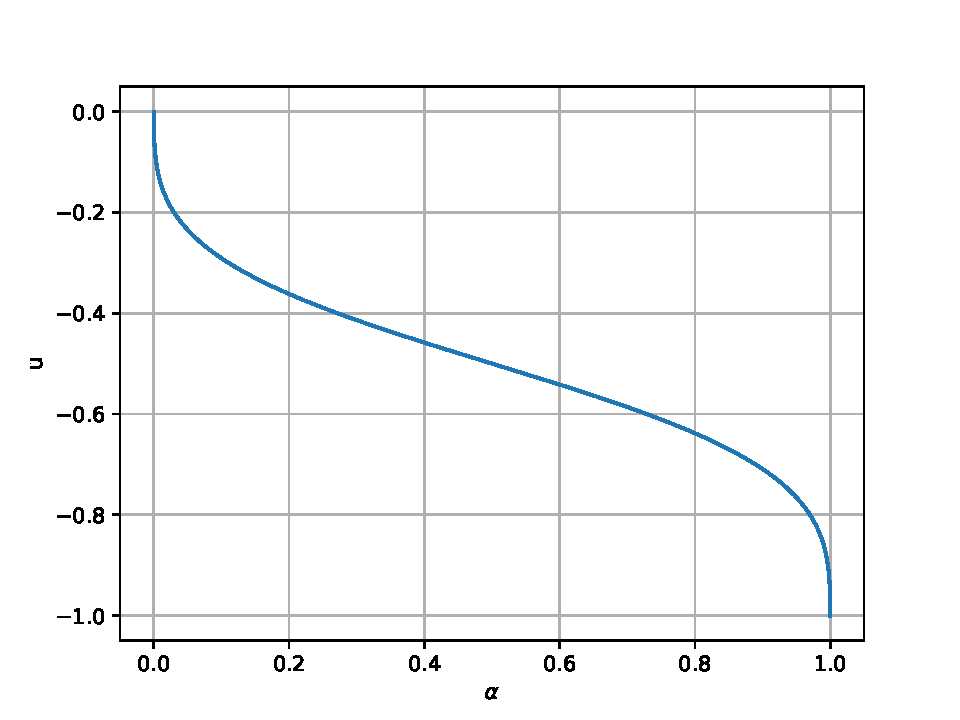
\includegraphics[scale=0.5]{../../Dev/DevPy/mipt/vpv/l1u.pdf}
\end{figure}
Соотвественно $x(\alpha)$:
\begin{figure}[H]
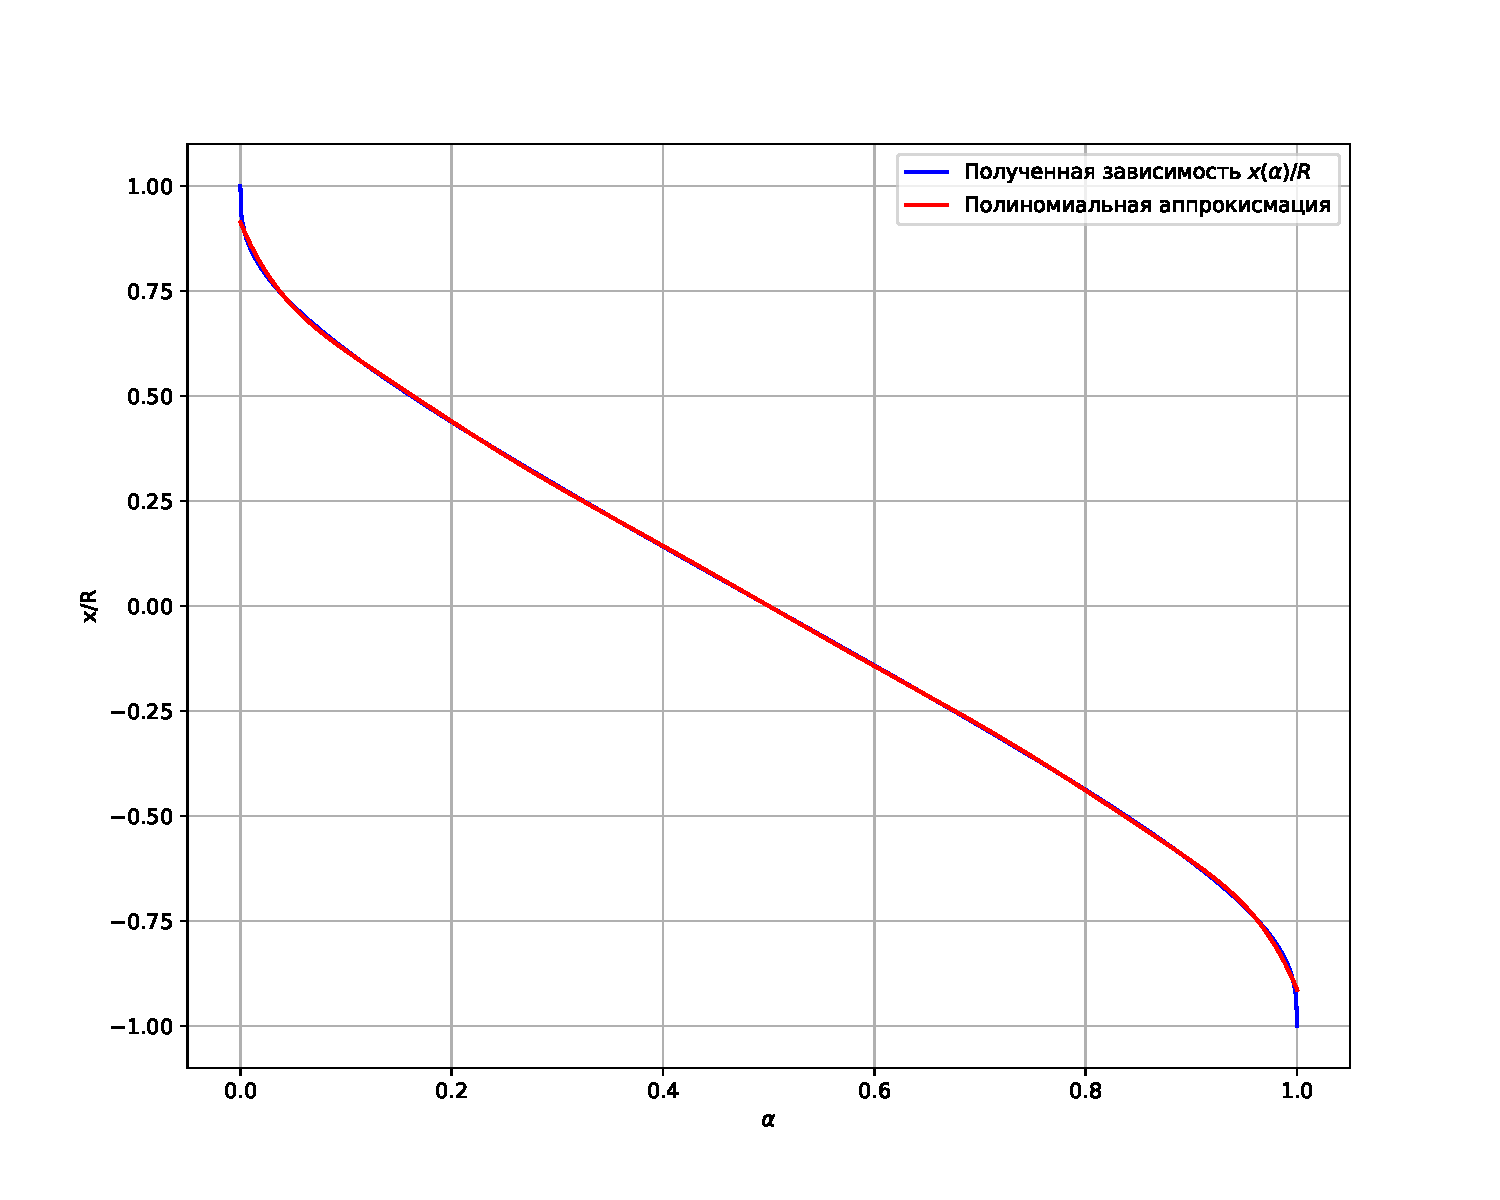
\includegraphics[scale=0.5]{../../Dev/DevPy/mipt/vpv/l1x.pdf} 
\end{figure}
В общем случае можем аппроксисмировать полученную зависимость с помощью многочлена 10-ой степени с коэфициентами $a_{10}...a_0 \text{ }(\text{индекс соответствует степени}) = ()$ с точностью $1.1\%$

Для $\alpha \ll 1$ подходит известное $x = R\left(1 - (\frac{\alpha}{3})^{\frac{1}{3}}\right)$:
\begin{figure}[H]
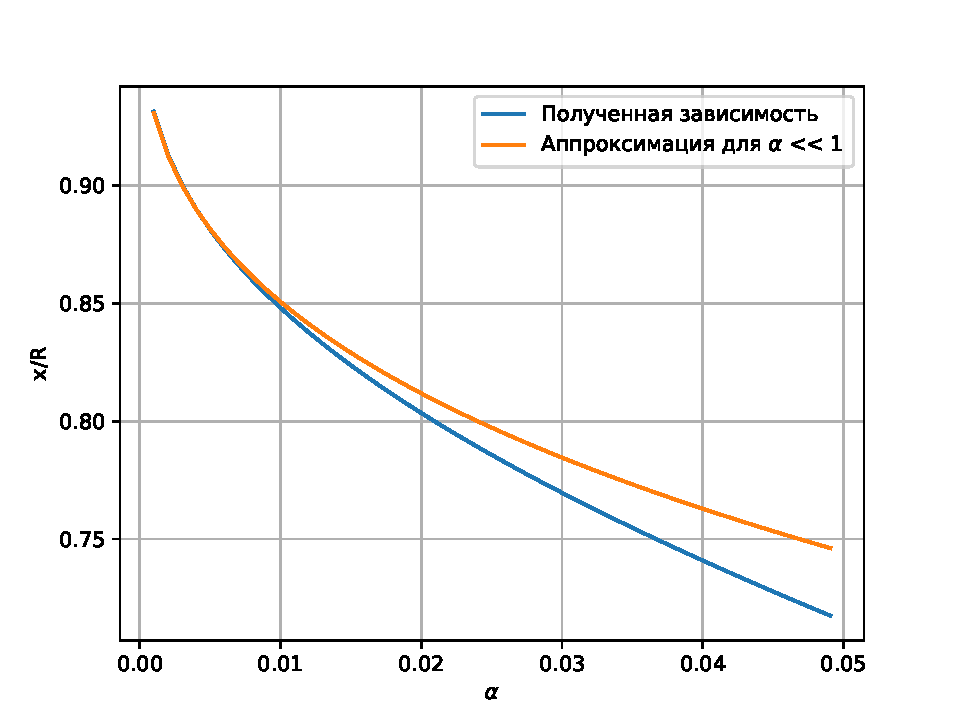
\includegraphics[scale=0.75]{../../Dev/DevPy/mipt/vpv/l1xsm.pdf} 
\end{figure}

\subsection{Точка $L_2$}
2-я точка Лагранжа соответствует случаю $s_0 = 1, s_1 = 1$. Получаем следующее решение:
\begin{figure}[H]
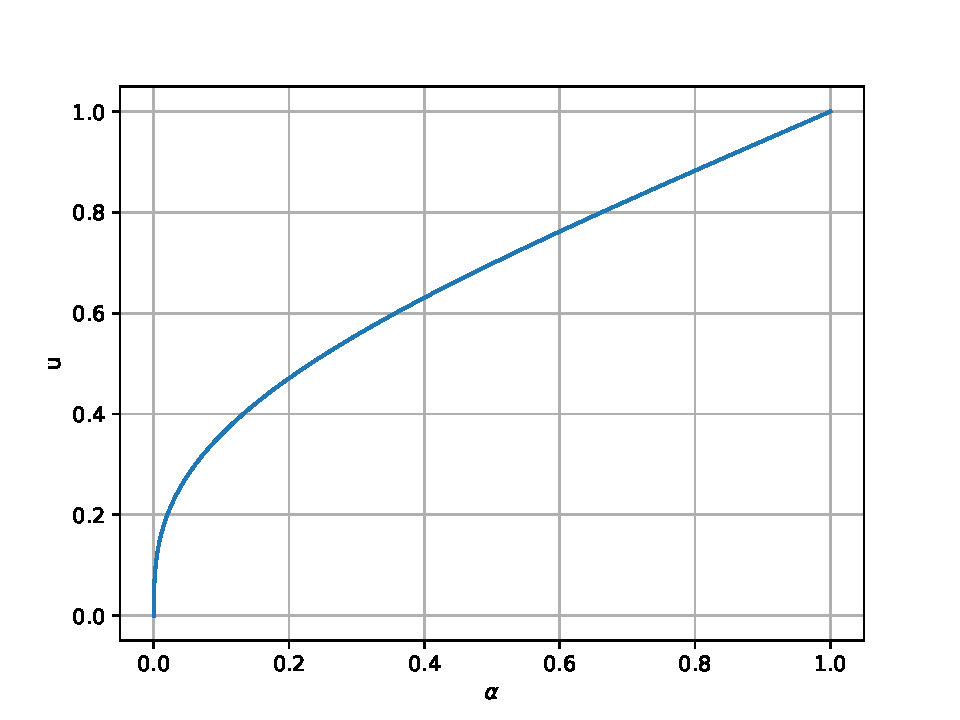
\includegraphics[scale=0.65]{../../Dev/DevPy/mipt/vpv/l2u.pdf}
\end{figure}
\pagebreak
Соотвественно $x(\alpha)$:
\begin{figure}[H]
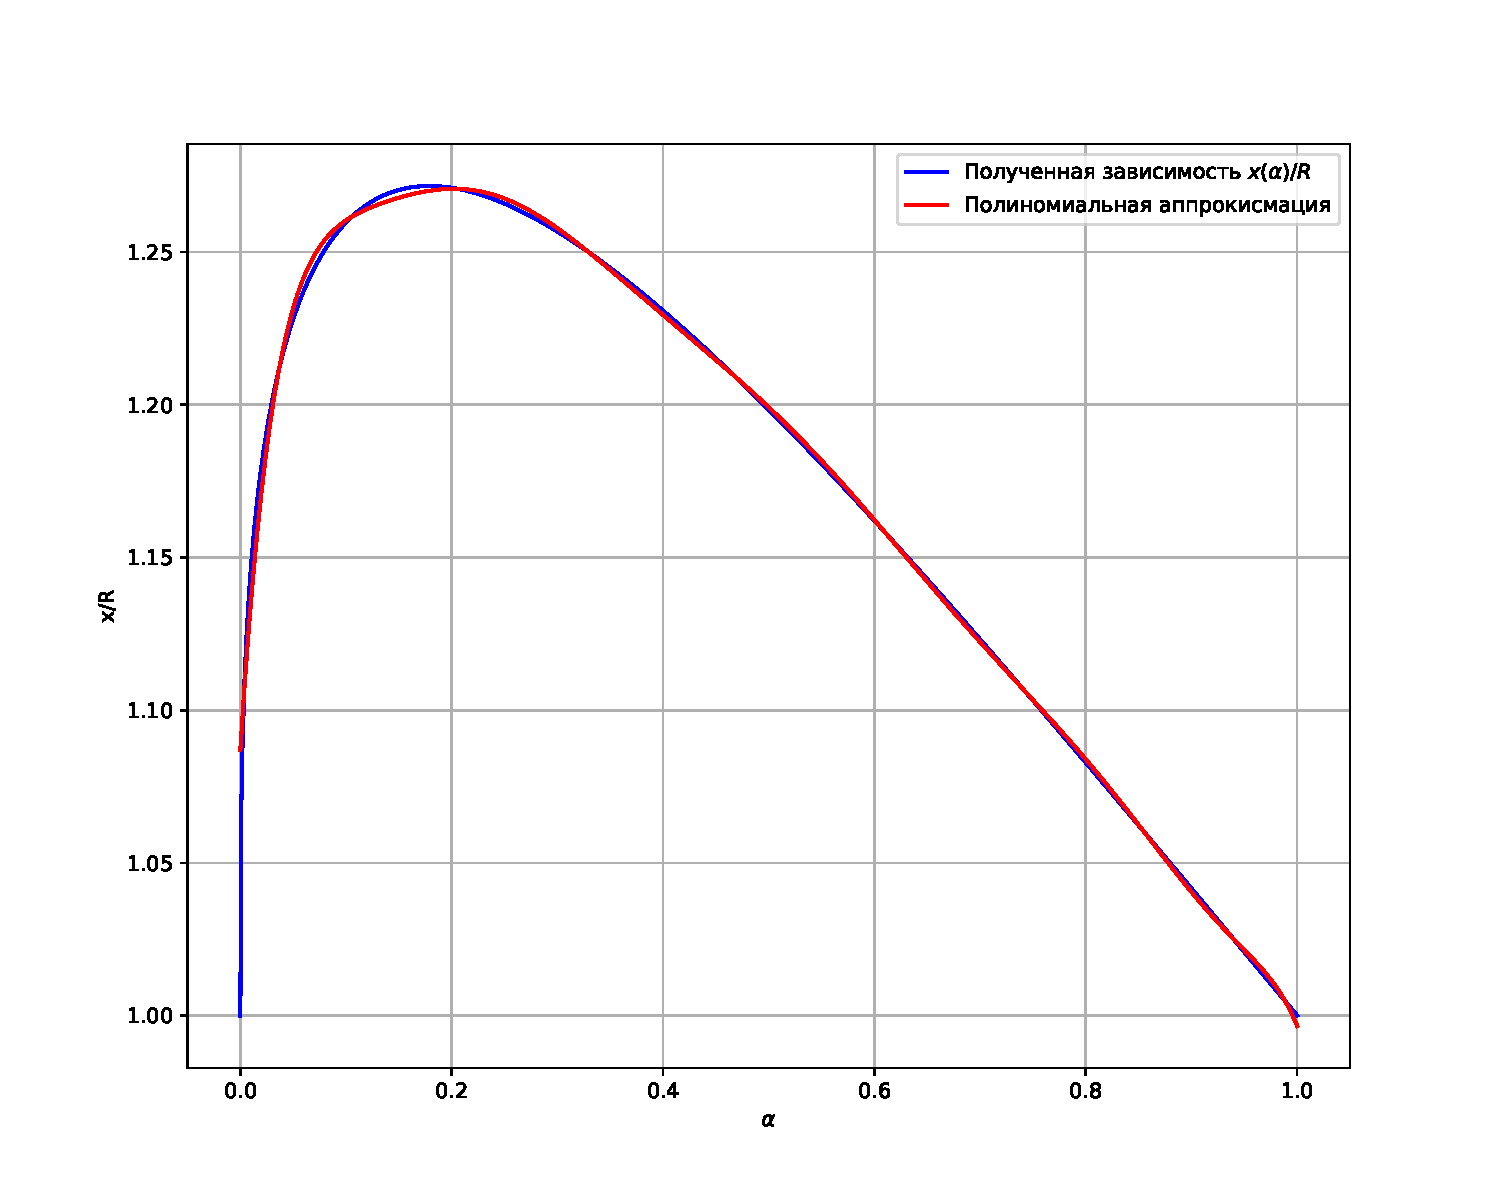
\includegraphics[scale=0.5]{../../Dev/DevPy/mipt/vpv/l2x.pdf} 
\end{figure}
В общем случае можем аппроксисмировать полученную зависимость с помощью многочлена 10-ой степени с коэфициентами $a_{10}...a_0 \text{ }(\text{индекс соответствует степени}) = ()$ с точностью $1.2\%$

Для $\alpha \ll 1$ подходит известное $x = R\left(1 + (\frac{\alpha}{3})^{\frac{1}{3}}\right)$:
\begin{figure}[H]
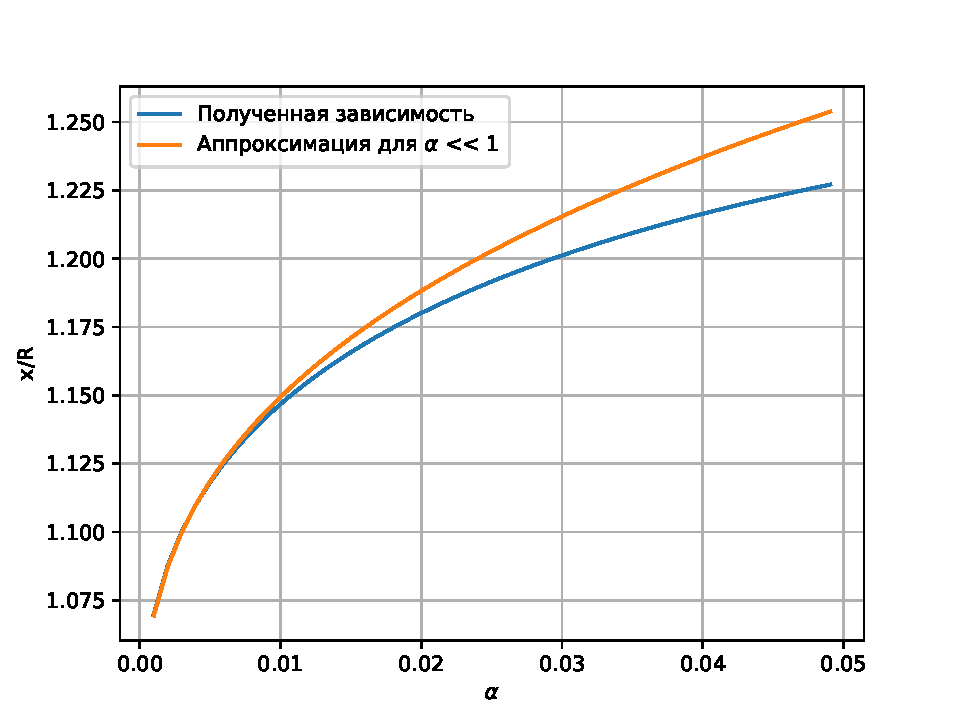
\includegraphics[scale=0.75]{../../Dev/DevPy/mipt/vpv/l2xsm.pdf} 
\end{figure}
\pagebreak

\subsection{Точка $L_3$}
3-я точка Лагранжа соответствует случаю $s_0 = -1, s_1 = -1$. Получаем следующее решение:
\begin{figure}[H]
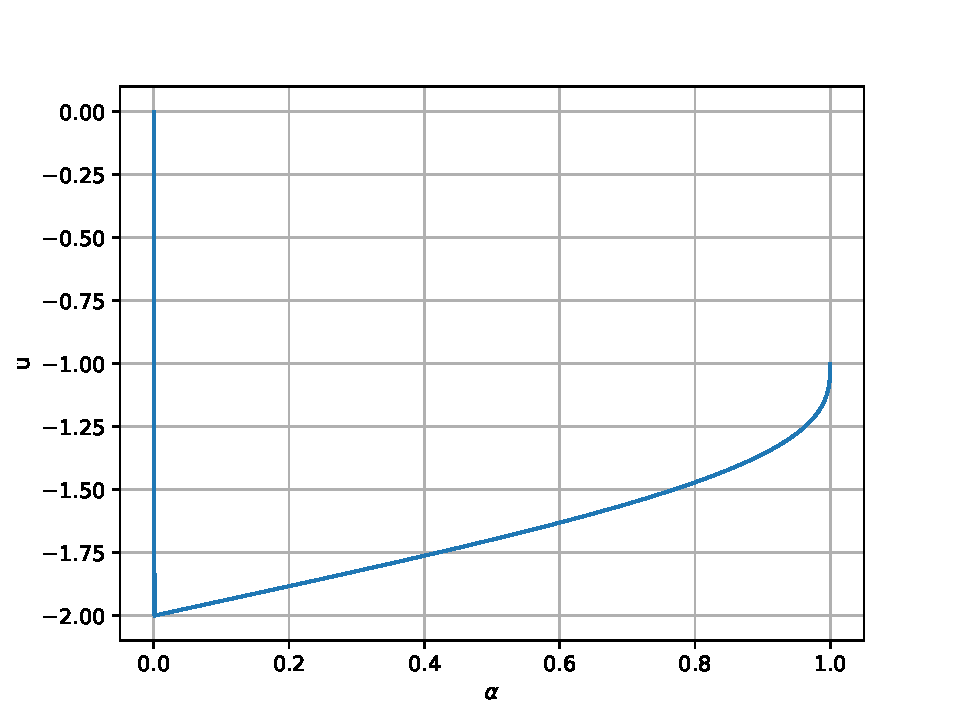
\includegraphics[scale=0.65]{../../Dev/DevPy/mipt/vpv/l3u.pdf}
\end{figure}

Соотвественно $x(\alpha)$:
\begin{figure}[H]
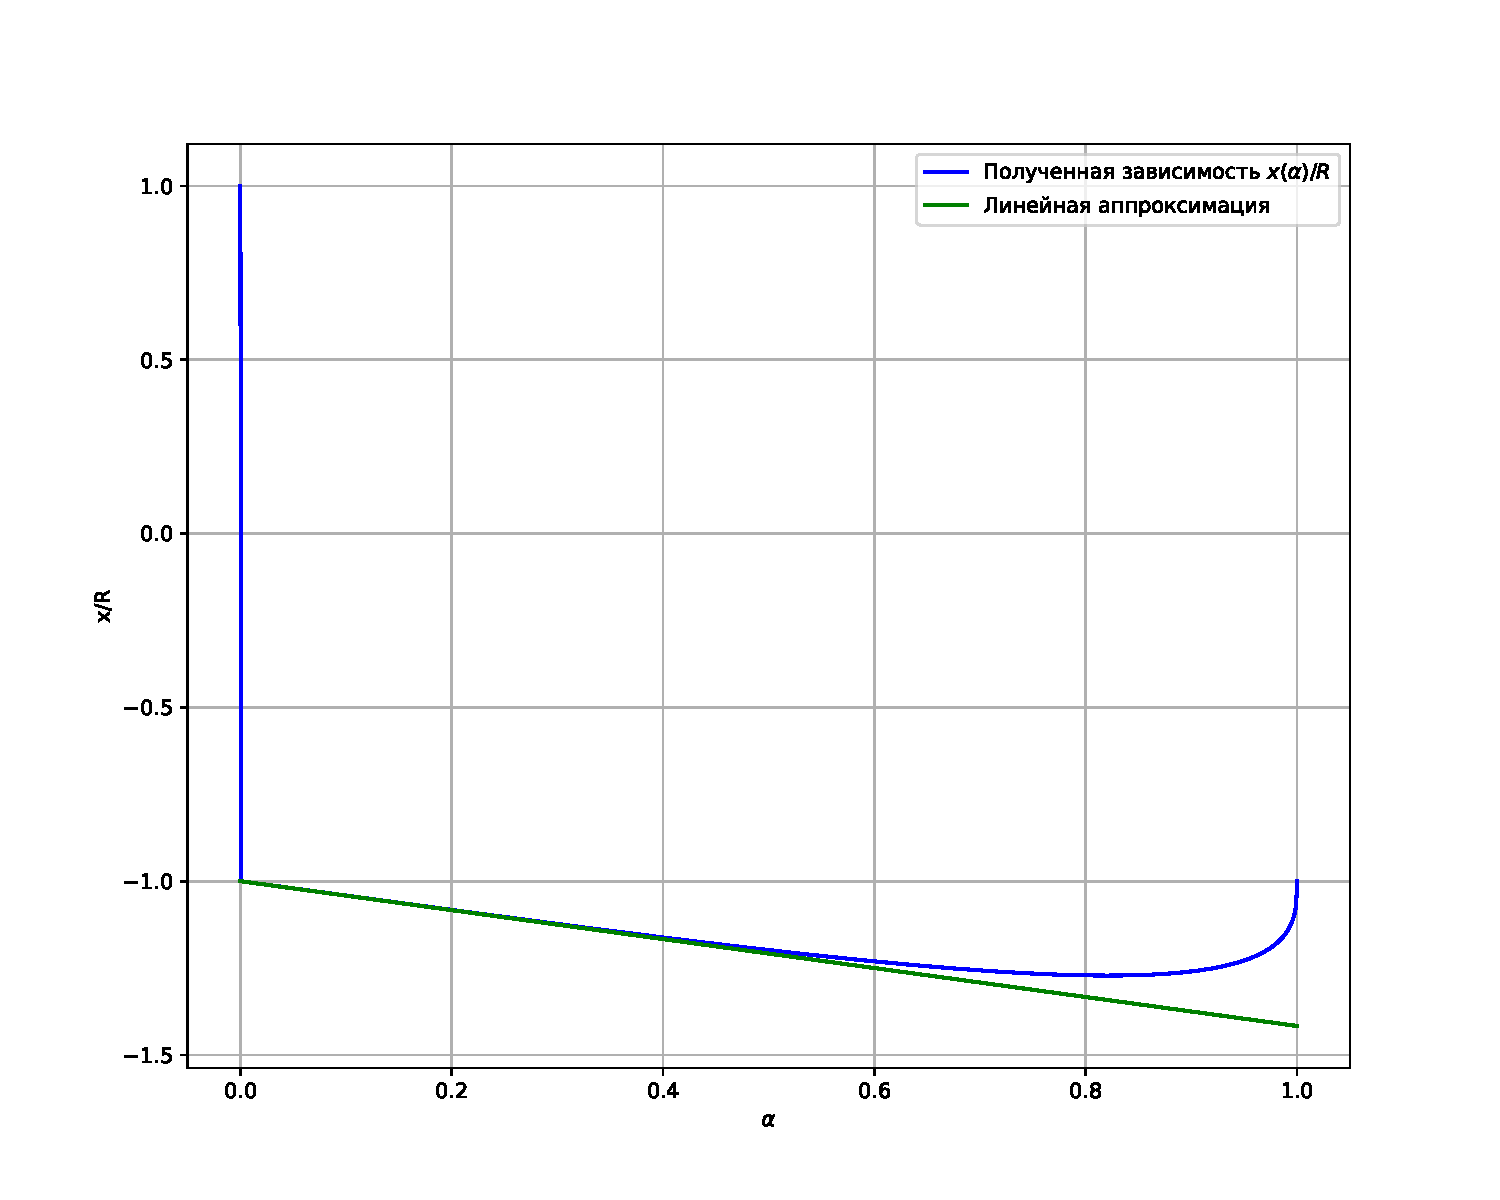
\includegraphics[scale=0.5]{../../Dev/DevPy/mipt/vpv/l3x.pdf} 
\end{figure}
Эту функцию аппроксисировать полиномом мы не будем, т.к. для $\alpha \le \sim0.5$ лучшей (и менее громоздкой) аппроксимацией будет $x = -R\left(1 + \frac{5}{12}\alpha\right)$

\section{Анализ устойчивости равновесия в точках Лагранжа}

Анализ равновесия положения заключается в определении того, как будет вести себя тело, при отклонении на малое расстояние от точки Лагранжа.

Мы будем рассматривать только плоское движение, тогда новые координаты тела при смещении от точки Лагранжа, можно записать как:
\begin{equation}
\begin{split}
&x = x_i + x_p \\
&y = y_i + y_p \\
&z = z_p
\end{split}
\end{equation}
Учитывая, что при отклонении от точки Лагранжа на тело будет дейтсвовать ненулевая сила Кореолиса, запишем \hyperref[8]{(8)} в следующем виде:
\begin{equation}
\ddot{\vec{r}} + 2(\Omega \times \frac{d\vec{r}}{dt}) = -\nabla(\varphi_G - \frac{1}{2}\Omega^2\vec{r}^2)
\end{equation}
Аргумент оператора набла в правой части называется псевдопотенциалом или обощенным потенциалом. Обозначим его как $U_\Omega$.

Записав это уравнение покомпонентно, пользуясь тем, что градиент псевдопотенциала в точке Лагранжа 0 (т.к. это точка экстремума псевдопотенциала), получим систему уравнений:
\begin{equation}
\begin{split}
\frac{d^2x_p}{dt^2} - 2\Omega\frac{dy_p}{dt} = -\frac{d^2U_\Omega}{dx^2}x_p - \frac{d^2U_\Omega}{dxdy}y_p - \frac{d^2U_\Omega}{dxdz}z_p \\
\frac{d^2y_p}{dt^2} + 2\Omega\frac{dx_p}{dt} = -\frac{d	^2U_\Omega}{dx^2}x_p - \frac{d^2U_\Omega}{dxdy}y_p - \frac{d^2U_\Omega}{dxdz}z_p
\end{split}
\end{equation}
Запишем её в матричном виде:
\begin{equation}
\frac{d}{dt}
\begin{pmatrix}
x_p \\
y_p \\
\frac{dx_p}{dt}\\
\frac{dy_p}{dt}
\end{pmatrix}
=
\begin{pmatrix}
0 & 0 & 1 & 0 \\
0 & 0 & 0 & 1 \\
\frac{d^2U_\Omega}{dx^2} & \frac{d^2U_\Omega}{dxdy} & 0 & 2\Omega \\
\frac{d^2U_\Omega}{dxdy} & \frac{d^2U_\Omega}{dy^2} & -2\Omega & 0
\end{pmatrix}
\begin{pmatrix}
x_p \\
y_p \\
\frac{dx_p}{dt}\\
\frac{dy_p}{dt}
\end{pmatrix}
\end{equation}
Если $\lambda$ - собственное значение линейного преобразования справа, то данное выражение эквивалентно:
\begin{equation}
\frac{dV}{dt} = \lambda V
\end{equation}
Решение данного уравнение известно: $V = ce^{\lambda t}$. Таким образом, если все собственные значения буду только мнимыми, система является затухающим осциллятором, т.е. в точке устойчивое равновесие. В ином случае величины отклонения будут экспоненциально расти, а значит в точке равновесие неустойчивое.

Для разных точек различаются только величины второй производной псевдопотенциала, которые можно получить непосредственно продифференцировав.

\textbf{Для $L_1$ и $L_2$ получим}:
\begin{equation}
\frac{d^2U_\Omega}{dx^2} = \pm 9\Omega^2, \text{ }\frac{d^2U_\Omega}{dy^2} = \pm 3\Omega^2, \text{ }\frac{d^2U_\Omega}{dxdy} = 0.
\end{equation}

По формуле $\lambda = \frac{\tau \pm \sqrt{\tau^2 - 4\Delta}}{2}$, где $\tau$ - след, $\Delta$ - определитель нашей матрицы получаем:
\begin{equation}
\lambda = \pm\Omega\sqrt{1 + 2\sqrt{7}}
\end{equation}

Таким образом, в $L_1$ и $L_2$ равновесие неустойчивое.

\textbf{Для $L_3$:}
\begin{equation}
\frac{d^2U_\Omega}{dx^2} = \pm -3\Omega^2, \text{ }\frac{d^2U_\Omega}{dy^2} =  \frac{7m_2}{8m_1}\Omega^2, \text{ }\frac{d^2U_\Omega}{dxdy} = 0.
\end{equation}

Отсюда:
\begin{equation}
\lambda = \pm\Omega\sqrt{\frac{3m_1}{8m_2}}
\end{equation}

Т.е. в $L_3$ равновесие неустойчивое

\textbf{Для $L_4$ и $L_5$:}
\begin{equation}
\frac{d^2U_\Omega}{dx^2} = \pm \frac{3}{4}\Omega^2, \text{ }\frac{d^2U_\Omega}{dy^2} =  \frac{9}{4}\Omega^2, \text{ }\frac{d^2U_\Omega}{dxdy} = \frac{3\sqrt{3}}{4}\gamma\Omega^2
\end{equation}
где $\gamma = \frac{m_1 - m_2}{m_1 + m_2}$

Получаем:
\begin{equation}
\lambda = \pm i\frac{\Omega}{2}\sqrt{2 - \sqrt{27\gamma^2 - 23}}
\end{equation}

Таким образом, в точках $L_4$ и $L_5$ равновесие будет устойчивым, если:
\begin{equation}
\gamma \ge \frac{23}{27} \text{ и } \sqrt{27\gamma^2 - 23} \le 2
\end{equation}

Второе условие выполняется всегда, а первое потребует:
\begin{equation}
m_1 \ge 25m_2\left(\frac{1 + \sqrt{1 - 4/625}}{2}\right)
\end{equation}

\section{Заключение}
Точки Лагранжа являются важным объектом в современной астрофизике. В частности, их свойства прямым образом используются для размещения в них космических обсерваторий ("Джеймс Уэбб" в $L_2$ или SOHO в $L_1$) для наблюдений как за дальним космосом, так и за нашей солнечной системой.

В нашей работе мы рассмотрели ограниченную задачу трех тел, нашли положение всех точек Лагранжа с помощью аналитических и численных методов, а также области корректного применения разных аппроксимаций. Кроме того, мы исследовали устойчивость равновесия каждой точки, что является довольно ценным результатом.
\end{document}